\documentclass[a4paper]{article}
\usepackage[utf8]{inputenc}
\usepackage[T1]{fontenc}
\usepackage{graphicx}
\usepackage{float}

\begin{document}
\pagenumbering{roman}
\title{Algorithmique et Bioinformatique \\ Assemblage de fragment \\ Rapport}
\author{Broh\'ee Jannou \& Ledru Santorin  \\ Groupe 12}
\maketitle
\begin{figure}[!htb]
\begin{center}
  
\includegraphics[width=\textwidth]{illustrations/UMONS_FS.jpg}
\end{center}
\end{figure}
\newpage
\pagenumbering{roman}
\renewcommand{\contentsname}{Table des matières}
\tableofcontents

\newpage
\pagenumbering{arabic}
\section{Introduction}

Le projet consistait à produire une séquence d'ADN cible en assemblant
une collection de divers fragments donnés en utilisant une approche
de type ``greedy''.

Pour arriver à produire cette séquence cible, on passe par plusieures
étapes:
\begin{itemize}
\item La recherche de l'alignement optimal entre chaque paire de fragments,
avec la méthode Semi-Global
\item La construction d'un graphe de chevauchement représentant le problème
\item La recherche d'un chemin hamiltonien dans ce graphe, correspondant
à une super-chaîne
\item Le consensus, levant les ambiguïtés restantes et alignant les fragments
les uns les autres
\end{itemize}
Dans la suite de ce rapport, nous expliquerons brièvement les choix
et les méthodes utilisées pour arriver au résultat et discuterons
ensuite de la qualités de ces résultats grâce à l'outil dotmatcher.

\newpage
\section{Implémentation}

\subsection{Représentation d'un Fragment et de son complémentaire}
\'Etant donné qu'un fragment d'ADN est constitué de 4 nucléotides différentes il nous est apparu qu'un byte était donc suffisant pour représenter un nucléotide. Connaissant la taille d'un fragment avant de vouloir le représenter, nous avons choisi de représenter un fragment comme étant un objet uniquement composé d'un tableau de byte. La représentation de son complémentaire inversé se fait par construction sur base du fragment initial . Nous parcourons le tableau de byte en commençant par la fin et nous inversons comme suite les nucléotides : A $\hookrightarrow$ T , T $\hookrightarrow$ A , C $\hookrightarrow$ G , G $\hookrightarrow$ C , GAP $\hookrightarrow$ GAP . Pour chaque nucléotide trouvé en position i dans le tableau , nous insérons son complémentaire en position lenght-(i+1) ou lenght représente la taille du fragment initial. De fait, comme nous commençons le parcours du tableau par la fin, le premier élément que nous inspection est en réalité de dernier et a comme indice i = (length-1). De la même manière, le premier élément dans le tableau se trouve à l'indice i = 0. L'opération  lenght-(i+1) = lenght-(lenght-1+1) =  0. Ainsi le nucléotide qui se trouve en dernière position dans le fragment initial sera complémenté avant d'être mis en première position dans le tableau du fragment représentant le complémentaire. Il en vas de même pour les autres nucléotide au positions restantes.  
\subsection{Graphe : sommet et arc}

A chaque sommet du graphe que nous allons créer, nous associons plusieurs informations que nous détaillons ici. 
Un sommet est un objet qui contient un fragment et 4 autre variable utilisées lors du chemin Hamiltonien, un boolean in qui représente un point d'entrée dans le fragment, un boolean inC qui représente un point d'entrée dans le complémentaire inversé fragment, un boolean out qui représente un point de sortie du fragment et un boolean outC qui représente un point de sortie du complémentaire inversé du fragment. 

En ce qui concerne les arc, ce sont des objets composés de 5 variables : int indexSommetSrc l'indice du sommet source, int indexSommetDst l'indice du sommet destination int score le score de l'alignement représenté par l'arc entre le fragment contenu dans le sommet destination et celui contenu dans le sommet source, un boolean srcC qui est vrai si on a pris le complémentaire inversé du fragment dans le sommet source false sinon et un boolean dstC qui est vrai si on a pris le complémentaire inversé du fragment dans le sommet destination false sinon. 

\subsection{Construction du graphe}
La construction des sommets est expliquée dans la section Parser. 
la construction des arcs se fait comme expliquer ici : pour l'ensemble de nos sommets (qui sont stockés dans une liste et ou l'indice d'un sommet corresponds à son indice dans cette liste), nous créons une tâche qui consiste à calculer tous les alignements possibles ( 8 pour chaque paire de fragments) entre le fragment contenu dans le sommet et les fragments contenus dans les sommets suivants dans la liste. Une fois cette tache créé, nous l'attribuons à un thread ( nous avons au total 2 fois le nombre de threads disponible sur une machine et ce afin de combler chaque petit "trous" entre les threads disponible sur la machine). Tous les threads renvoient le résultat de leurs taches dans une seule et même file. Une fois que tous les threads ont finis leur travail, nous insérons le contenu de la file dans notre arc. La raison pour laquelle chaque thread ne renvoie pas directement les résultats obtenus dans le graphe est qu'il y aurait un phénomène de concurrence sur l'accès au graphe.  


\subsection{Parser}
Nous nous basons sur le format de représentation d'un fragment dans un fichier fasta afin de repérer les différents fragments. Pour ce faire nous faisons la distinction entre les lignes commençants par le caractère '>' et les autres ligne contenants les nucléotides du fragment, nous commençons donc par repérer la première ligne commençant par le caractère mentionné et passons a la ligne suivante, nous enregistrons l'intégralité de cette ligne et passons à la ligne suivante. nous réitérons ce processus jusqu'au moment ou nous arrivons à une ligne qui commence par le caractère '>'. A ce moment nous savons que nous venons de lire un Fragment que nous enregistrons directement dans un sommet du graphe. nous procédons ainsi jusqu'à ce que nous arrivions à la fin du fichier et nous enregistrons le dernier fragment dans le graphe. 


\subsection{Tri}
Pour trier les arcs par score décroissant nous avons opté pour un tri grâce à la méthode sort de la Classe Collection des librairies de base de Java.

\subsection{Chemin Hamiltonien}

La méthode pour trouver un chemin hamiltonien dans le graphe de chevauchement
est une méthode greedy, celà signifie simplement qu'on affecte un
score aux différents choix possible et qu'on envisage toujours le
choix de score maximal en premier. L'algorithme procède comme suit:
\begin{itemize}
\item On crée autant d'ensembles (Set) qu'il y a de sommets dans le graphe
\item On ajoute un sommet par ensemble
\item on considère l'arc de score maximal, si les sommets considérés n'ont
pas déjà été séléctionnés et s'ils appartiennent à des ensembles différents,
on merge leurs ensembles, on sélectionne l'arc, on bloque les sommets
comme sélectionnés respectivement en entrée et en sortie et on bloque
égalements leurs complémentaire (booléens)
\item sinon, on passe à l'arc suivant
\item jusqu'à ce qu'il ne reste plus qu'un seul ensemble, celà signifie
qu'on a sélectionné tous les sommets
\end{itemize}

\subsection{Consensus}

Tout d'abord, pour le consensus, on change un petit peu la manière
de représenter les fragments. En observant les fragments, nous avons
remarqué qu'en les alignant les uns les autres, on ajouté un très
grand nombre de gaps en début et en fin de chaînes. Nous avons donc
décidé pour le consensus de permettre de représenter le fragment sous
forme ``courte'' en otant tous les gaps de début et de fin de chaîne
et en maintenant le nombre de gaps de début et de fin dans des variables.
celà permet de parcourir juste la partie contenant les nucléotides
des fragments et évite de parcourir un grand nombre de gaps pour rien
(En pratique celà rend le consensus de l'ordre de mille fois plus
rapide).

Nous utilisons un vote de majorité pour effectuer le consensus, en
maintenant une liste de compteurs pour chaque indice de la chaîne
finale. Le consensus se déroule comme suit:
\begin{itemize}
\item On parcours les arcs du chemin hamiltonien, pour le premier, on ajoute
directement les sommet source et destination aux compteurs du vote
de majorité, et on maintient la destination dans une variable nommée
lastFrag
\item On passe à l'arc suivant, on compare lastFrag au sommet source de
l'arc et s'il sont différents, on propage les gaps, dans les deux
sens, c'est à dire que si on a un gap dans le fragment, mais pas dans
le lastFrag, on ajoute un compteur vide à l'indice en question et
si c'est l'inverse, on ajoute un gap au fragment, ainsi qu'au fragment
destination de l'arc.
\item On ajoute le fragment destination au vote de majorité (le source y
est déjà de part l'étape précédente) et on passe à l'arc suivant
\item Une fois qu'on a traité tous les arcs, on vérifie les compteurs et
on renvoie la valeur la plus retrouvée par indice(sans compter les
gaps), si on a une égalité, on choisit aléatoirement parmis les résultats
maximums\end{itemize}

\section{Résultats}


\subsection{Collections simplifiées}

Nous intégrons ici quelques résultats sur des collections simplifiées,
ne contenant pas de fragments complémentaires inversés pour montrer
que les résultats obtenus sur celles-ci sont satisfaisants


\subsubsection{Collection 1}

On peut voir ici qu'on à une droite bien pleine avec juste quelques
points par-ci, par-là, dénotant d'une adéquation presque parfaite
avec la cible.

\begin{figure}[H]
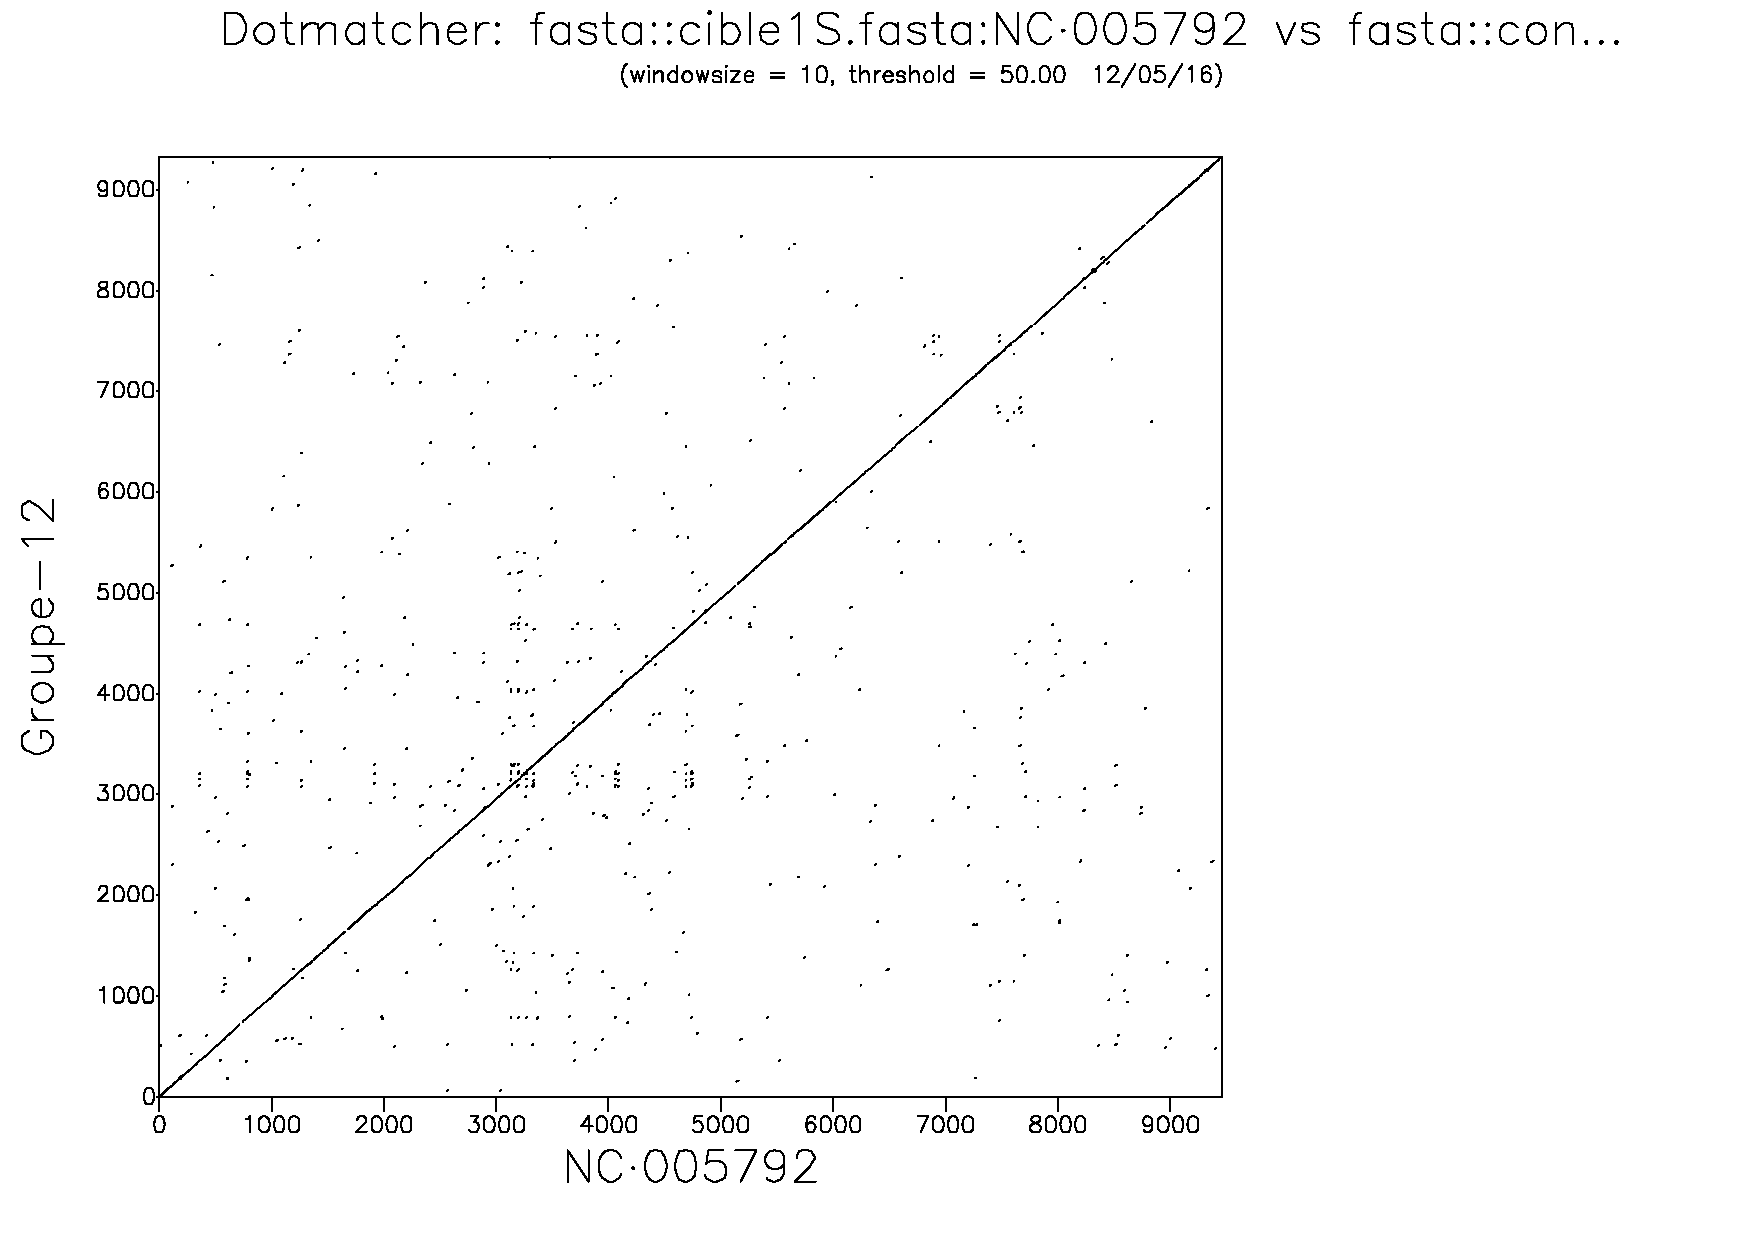
\includegraphics[scale=0.4]{1S}\caption{Dotmatcher Collection simplifiée 1}
\end{figure}



\subsubsection{Collection 2}

Ici encore, on obtient de bon résultats, sur une collection bien plus
grosse, avec cette fois une micro coupure dans la droite et beaucoups
plus de points épars.

\begin{figure}[H]
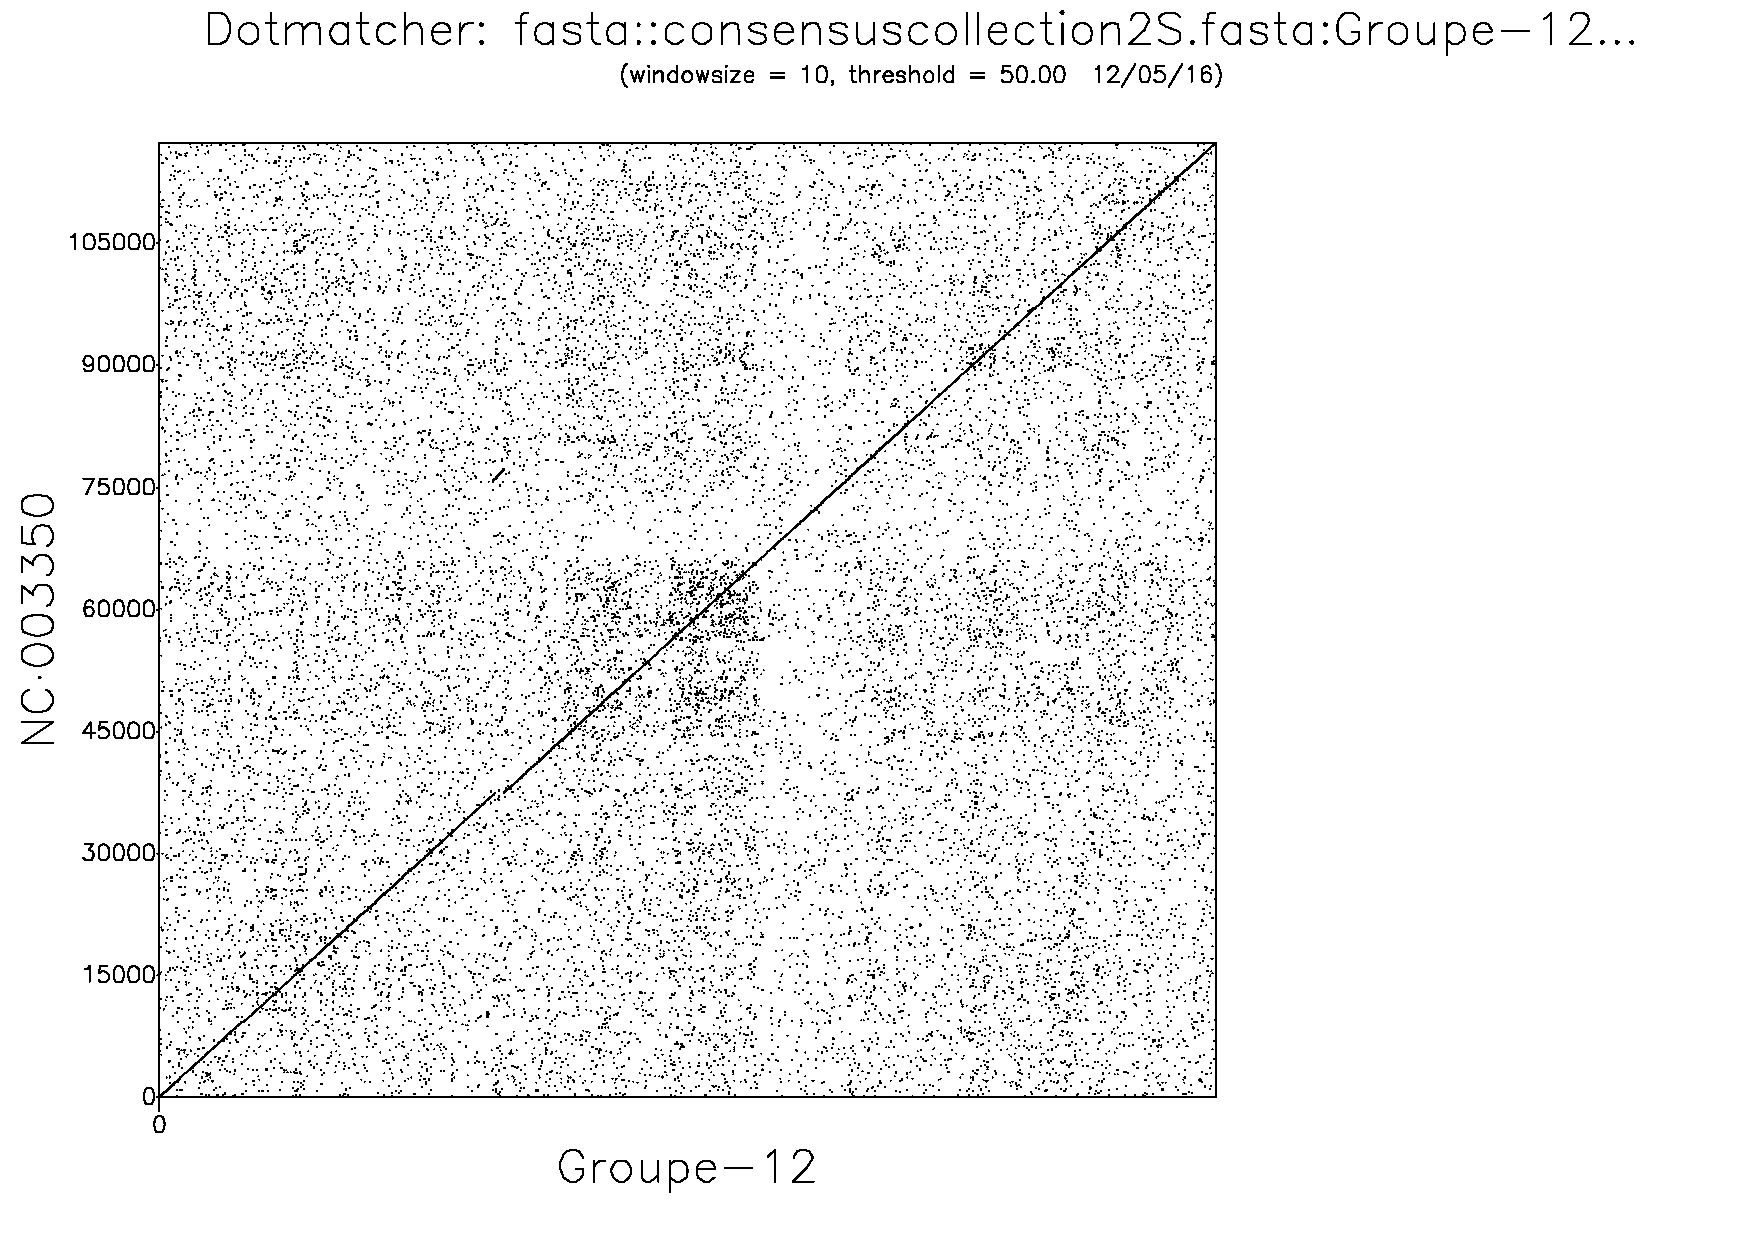
\includegraphics[scale=0.4]{2S}\caption{Dotmatcher Collection simplifiée 2}
\end{figure}



\subsection{Collections avec complémentaires inversés}

Pour les collections prenant en compte les complémentaires inversés,
notre programme s'en sort moins bien, avec des résultats imparfaits.
Les graphes montrent à chaque fois d'abord le dotmatcher résultant
de la comparaison avec le résultats du consensus, puis avec le complémentaire
inversé de celui-ci.


\subsubsection{Collection 1}

On voit pour cette collection qu'on obtient une adéquation plutôt
bonne avec la cible, avec un résultats plutôt grand quand même (14000
nucléotides contre 10000 pour la cible) et quelques morceaux éparpillés.

\begin{figure}[H]
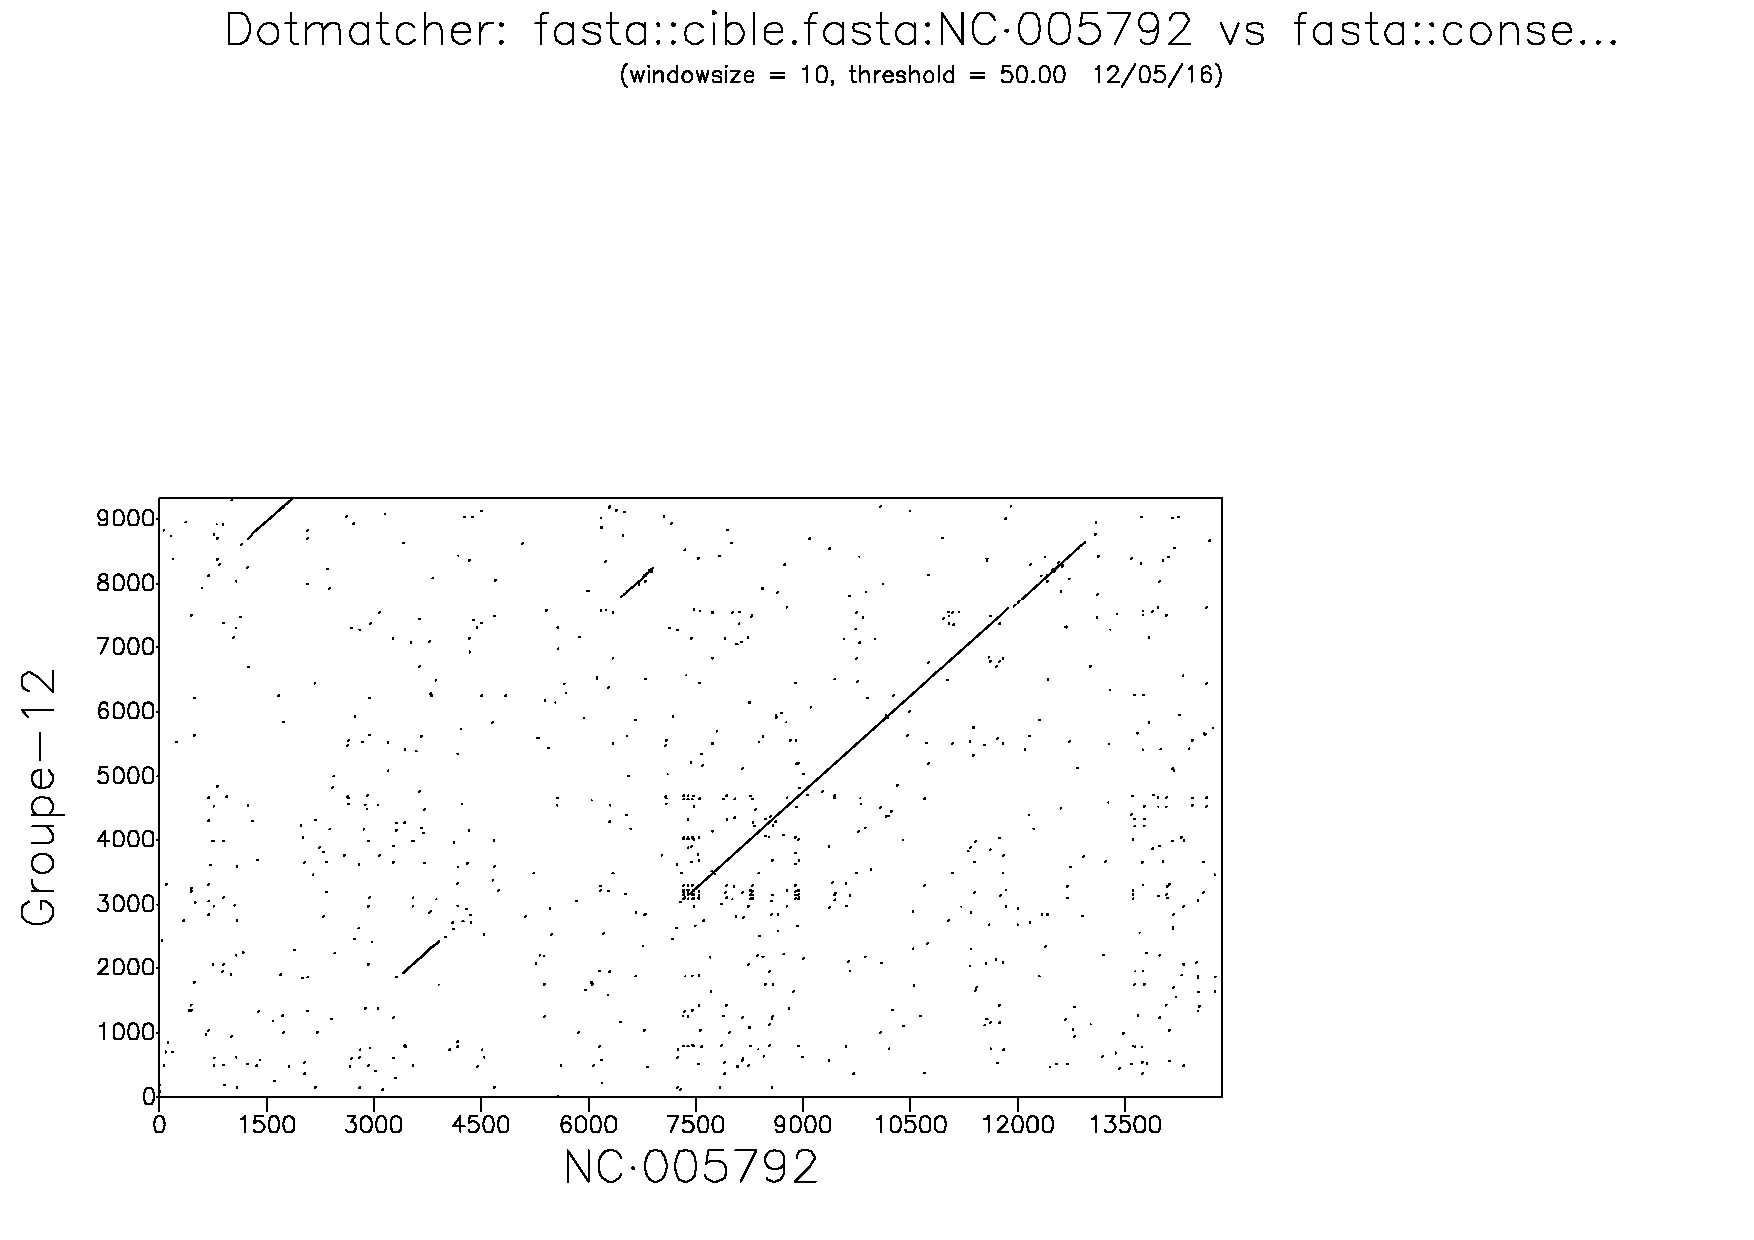
\includegraphics[scale=0.25]{1}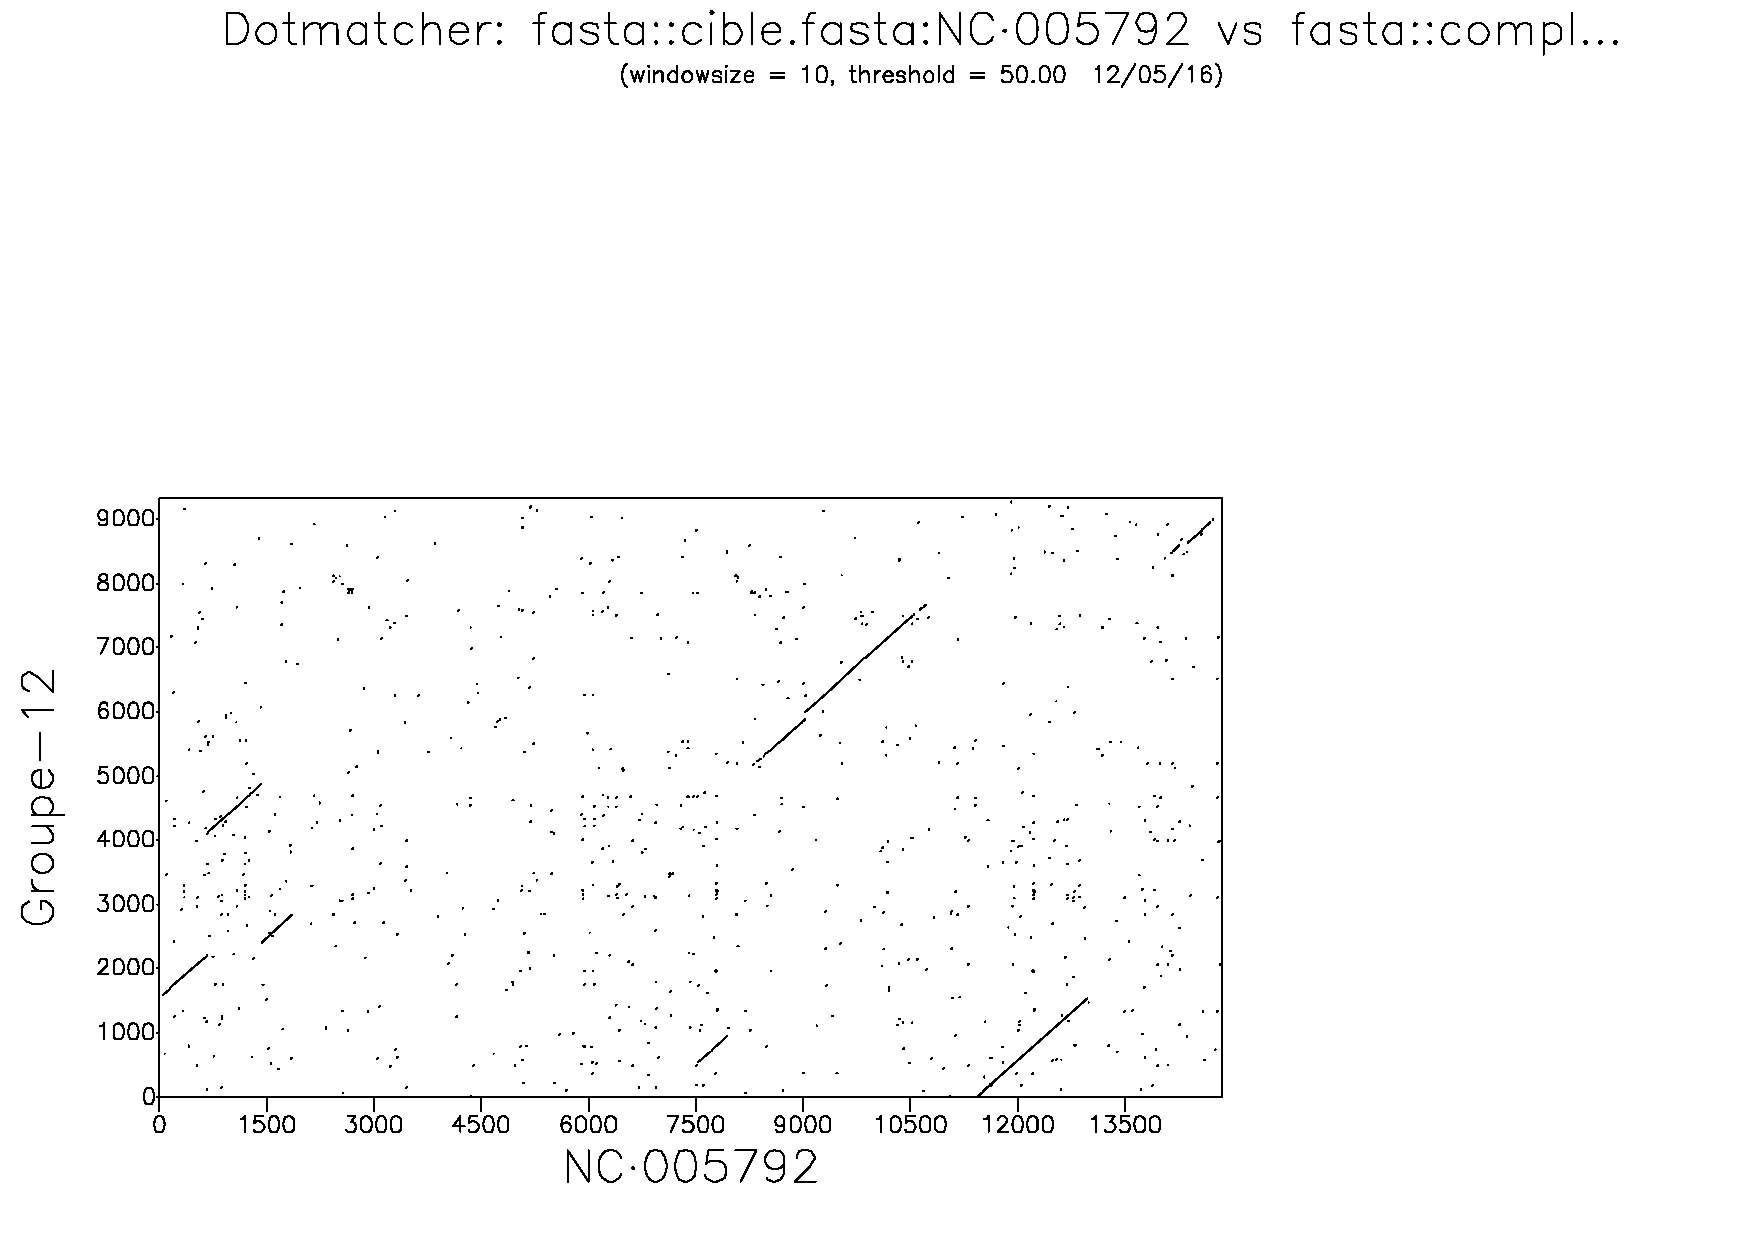
\includegraphics[scale=0.25]{1compl}\caption{Dotmatcher Collection1}
\end{figure}



\subsubsection{Collection 4}

On obtient ici un résultat plutôt bon mais morcelé, avec encore une
fois un résultat de trop grande taille par rapport à la cible.

\begin{figure}[H]
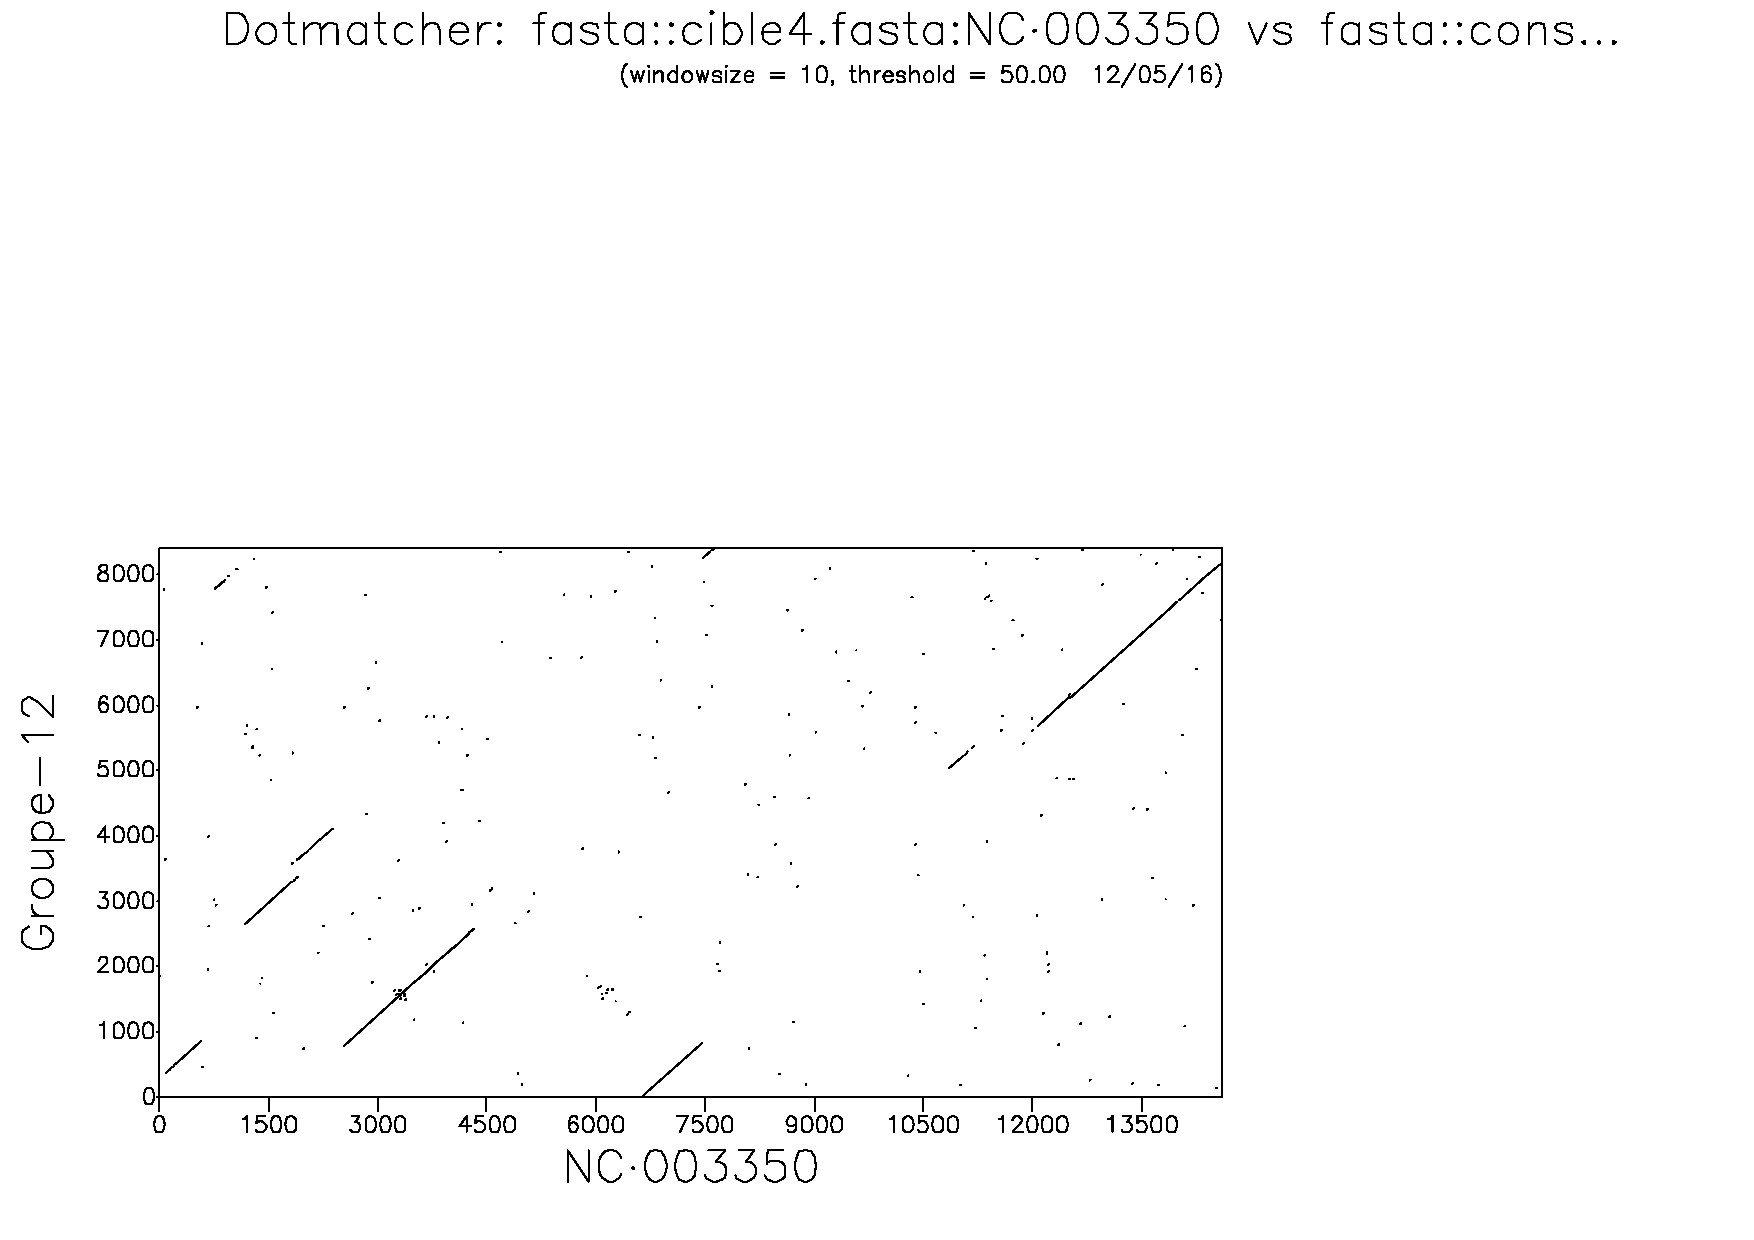
\includegraphics[scale=0.25]{4}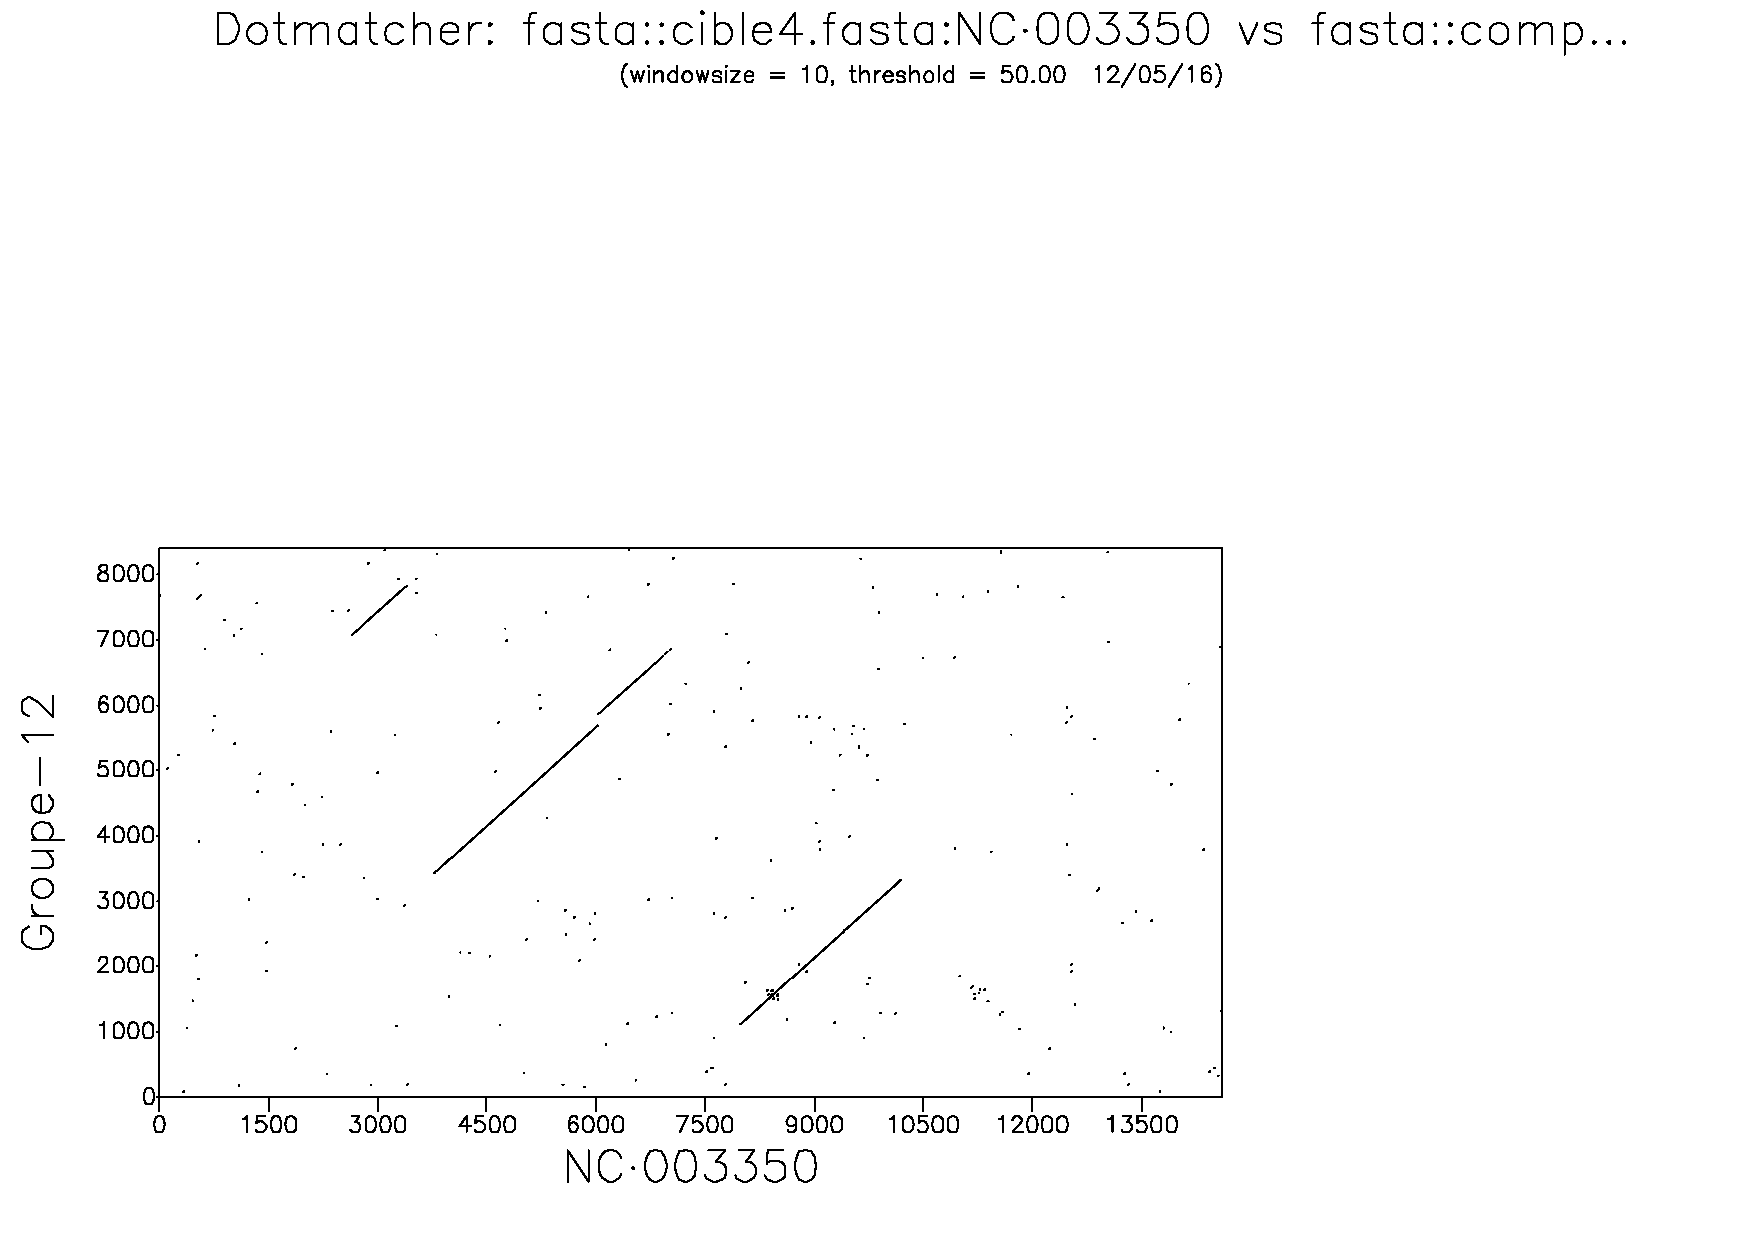
\includegraphics[scale=0.25]{4compl}\caption{Dotmatcher Collection 4}
\end{figure}



\subsubsection{Collection 5}

Comme pour les collections de taille similaire, on obtient un résultat
morcelé et un peu grand pour la cible.

\begin{figure}[H]
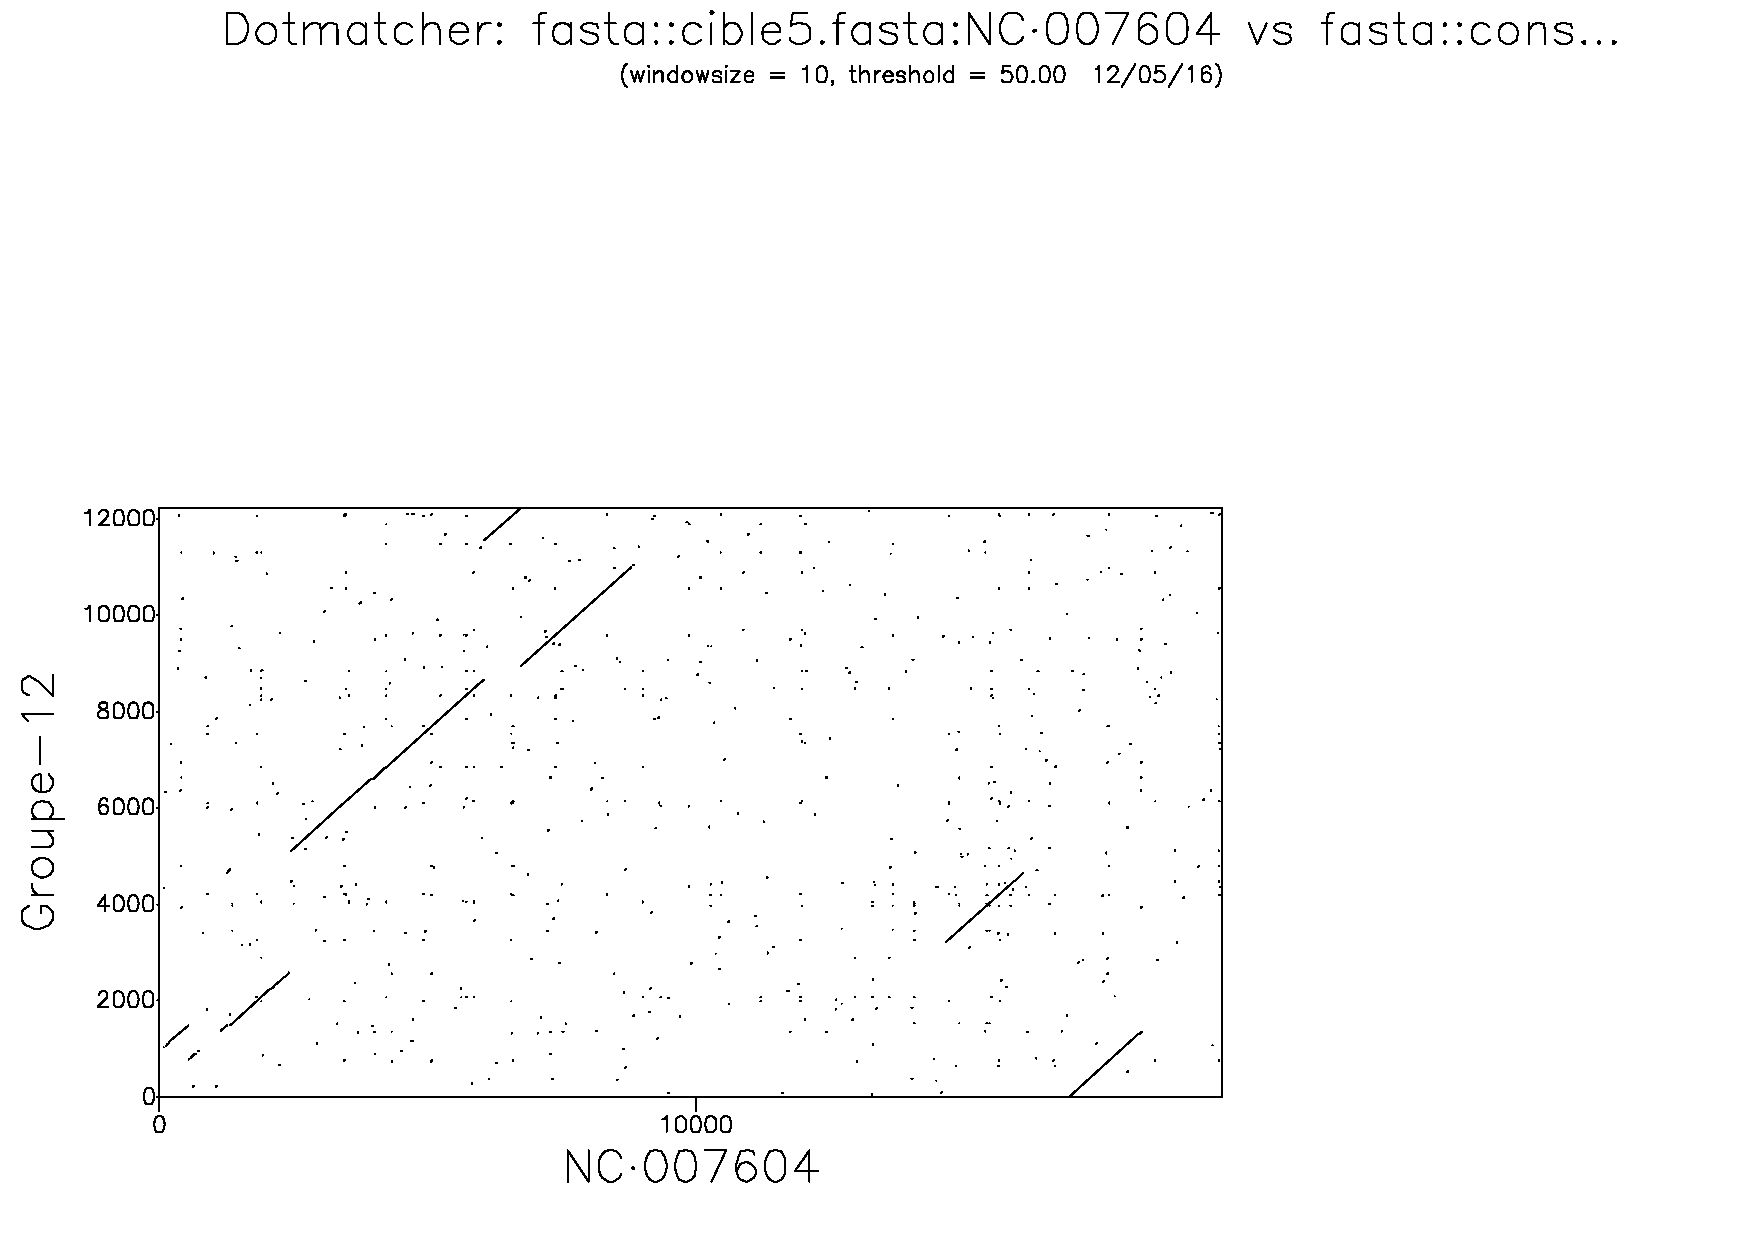
\includegraphics[scale=0.25]{5}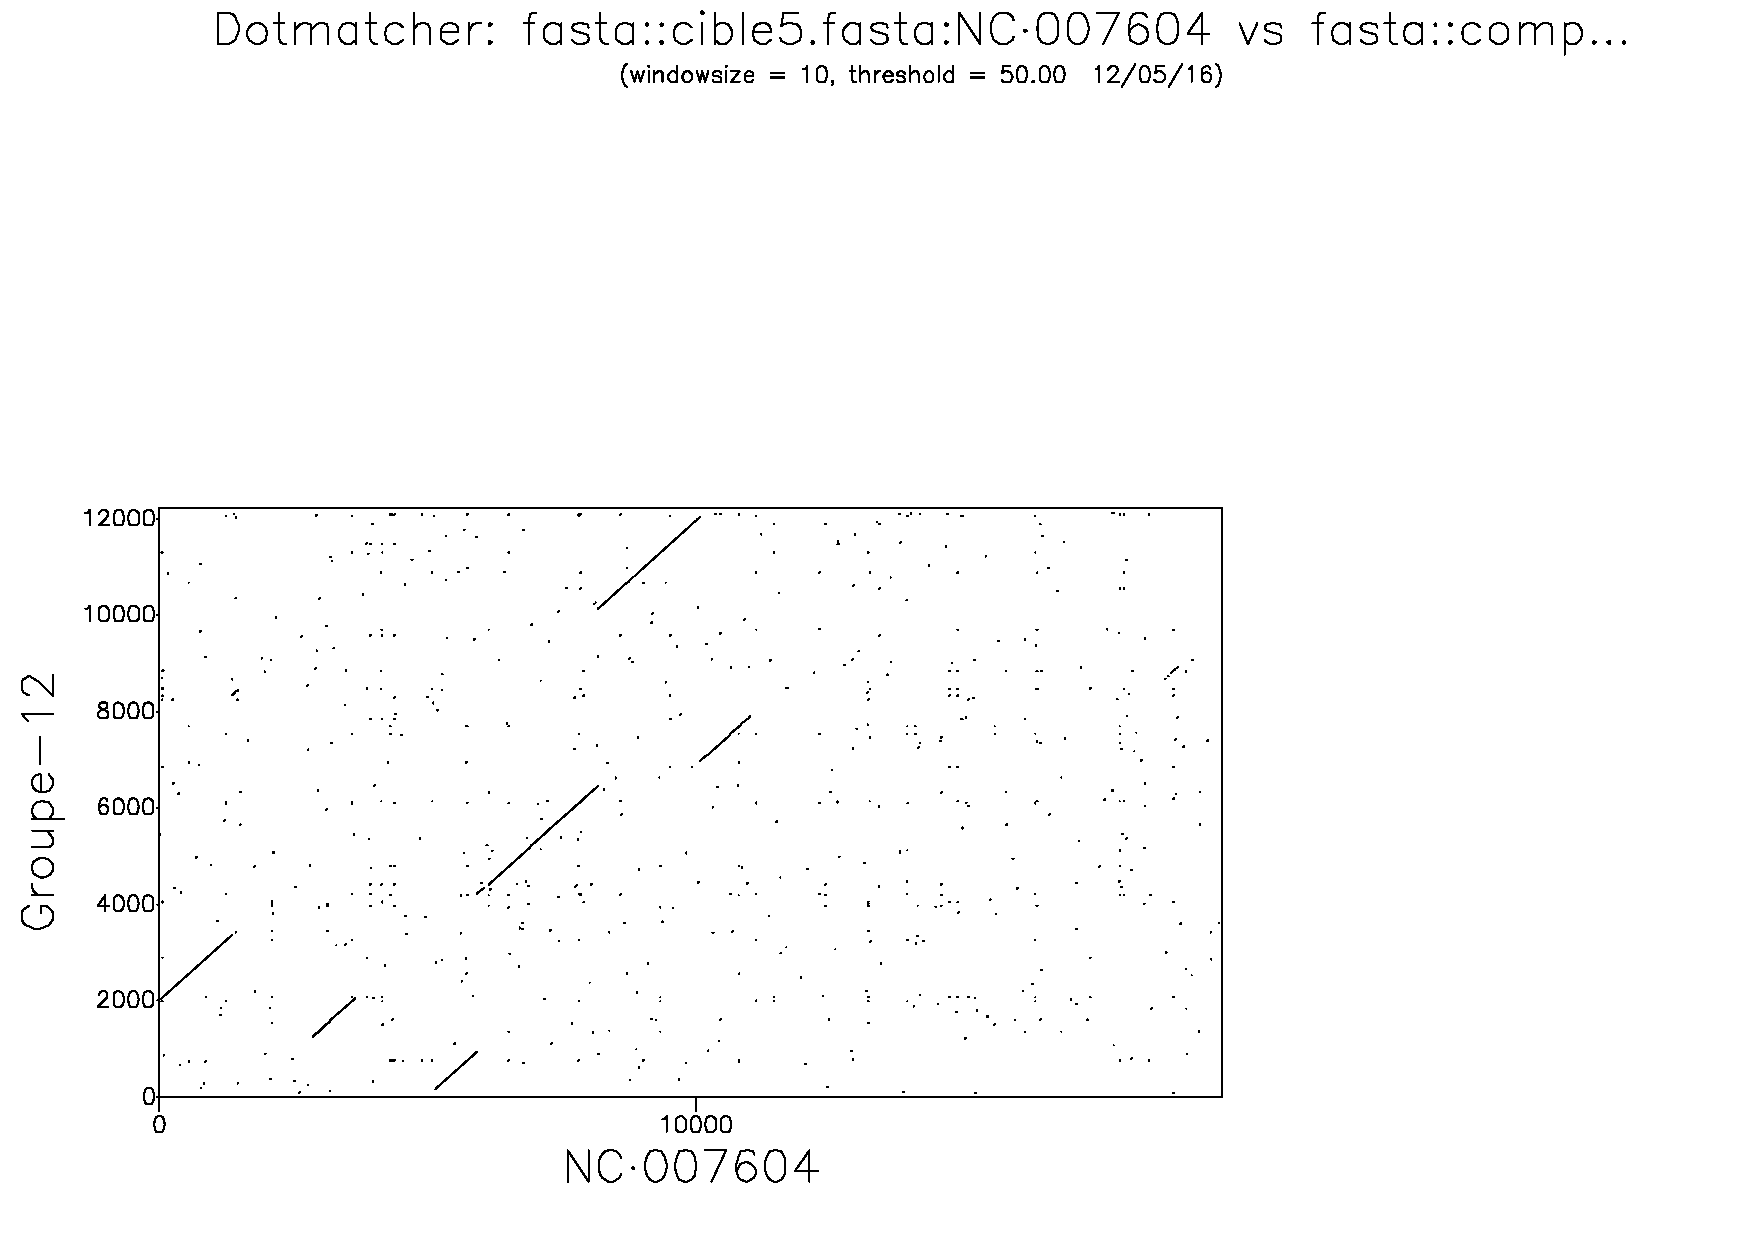
\includegraphics[scale=0.25]{5compl}\caption{Dotmatcher Collection 5}
\end{figure}

\section{Conclusion}
Ce projet nous a permis de nous familiariser quelques peu avec la notion de séquençage ADN et la Bioinformatique.

Nous avons rencontré quelques difficultés lors de l'implémentation du projet, mais ce fût très intérressant car il s'agissait d'un des premiers projets très gourmand en ressources et où l'optimisation, autant au niveau de la mémoire que du temps était primordiale pour pouvoir obtenir des résultats.

En ce qui concerne nos résultats, ils ne sont pas parfaits et le projet mériterait encore quelques modifications, notamment au niveau de la taille de certaines séquences cibles, mais nous sommes quand même fiers de ce que nous avons accompli.
\end{document}
